\chapter{Dark Matter Detection}

\section{Overview}
In the previous chapter, we've established that the overall scientific community believes that dark matter
probably consists of some particle. Here, we will discuss some of the current experiments and initiatives
launched by the scientific community to determine the identity of dark matter. 

As mentioned in the previous section, most scientists believe that dark matter exists in the form of WIMPs.
Because WIMPs are a stand-in for a very large class of particles, they also occupy a very large range of
masses, from as small as \( 1 \, \mathrm{GeV / c^2} \) all the way to \( 10^{5} \, \mathrm{GeV / c^2} \).
This poses somewhat of a problem when it comes to designing an experiment to detect such particles, as there
is no single detector that's going to be able to cover this entire range of energies. Instead, what
researchers do is focus on a particular range of masses, and try to detect particles within that range. To
this end, there are three primary ways that experiments go about detecting WIMPs: either we generate them at
particle accelerators (like the LHC), we detect them directly from astronomical sources like the sun and
other galaxies high in dark matter, or we detect their scattering interactions in low-background experiments.
This last method is the one that is of interest in this thesis, and it is the one that we will focus on for
the rest of the discussion.  


\section{Collision based DM Detection}
Collision based detection refers to the process of designing an experiment where we deliberately prepare an
experimental sample, with the objective of essentially waiting until a dark matter particle interacts with
the sample. This will cause a brief but detectable signal, which is then picked up using various instruments.
The actual physics behind the detectors is rather complicated, so we will only dive deeper into two
particular instruments (see \cref{TES} and \cref{KID}). For now though, we will focus on giving a
general overview of how these collision based detection methods help us confirm and find the identity of dark
matter. In this section, much of the content is derived from \cite{schumannDirectDetectionWIMP2019}.

To begin, we use the following formula to calculate the expected rate that a WIMP scatters off a nucleus with
mass \( m_N \):
\begin{equation}
	\label{expected-scatter}
	\dv{R}{E_\text{nr}} = \frac{\rho_0 M}{m_n m_{\chi}} \int_{v_\text{min}}^{v_\text{esc}} v f(v)
	\dv{\sigma}{E_\text{nr}} \diff v
\end{equation}
Here, \( \rho_0 \) is the local dark matter density, \( M \) is the target mass of the detector; \(
m_{\chi} \) is the mass of the WIMP; \( \sigma \) is the scattering cross section and \( f(v) \) is the
velocity distribution of the WIMPs; \( E_\text{nr} \) is the "nuclear recoil" energy -- essentially the
energy imparted to the target nucleus by the WIMP. Essentially this is just the same formula as the standard
form for expectation:
\[
	\mathbb E[X] = \int_{-\infty}^{\infty} x P(x) \diff x
\]
where \( P(x) \) represents the probability distribution we are interested in. \( v_\text{min} \) is
calculated using the following formula:
\begin{equation}
	\label{v-min}
	v_\text{min} = \sqrt{\frac{E_\text{nr}m_N}{2} \frac{1}{\mu^2}}
\end{equation}
% should I try to explain this formula or not? 
Here \( \mu \) represents the reduced mass of the WIMP and nucleus. The physics of how \cref{expected-scatter} and
\cref{v-min} are derived is too complex for this discussion; the objective of including
this formula is to make the point that \( v_\text{min} \) is nonzero, so there is a minimum threshold energy
that WIMPs must have for them to be energetic enough to be picked up by our detector. The more interesting
thing about \cref{expected-scatter} is that there is a maximum velocity \( v_\text{esc} \) that we
are concerned with. The reason for this is because while our detector will be able to detect WIMPs at
velocities higher than this, their velocity being above the escape velocity of the Milky Way means that they
are not dark matter particles that are bound by the Milky Way, and thus we are not interested in those
detections.  

With the equations in place, we turn to one of the central equations we will concern ourselves with: 
\[
	N = T \int_{E_\text{low}}^{E_\text{high}} \epsilon(E_\text{nr}) \dv{R}{E_\text{nr}} \diff E_\text{nr}
\]
\( \epsilon \) is the efficiency of the detector at the energy. This equation is actually rather simple, as
it is just the product of \( T \) and the rate of detection, which is given by the integral. It is weighted
by the detector efficiency, since physical detectors are imperfect. This equation is extremely important to
understanding the detector, since \( N \) is the quantity we ultimately measure in our experiment. What this
equation really tells us is that in order to understand \( N \), we need to have a very good understanding of
our experimental setup, since \( \epsilon(E_\text{nr}) \) is crucial to determining \( N \). Obviously, \(
\epsilon(E_\text{nr}) \) will differ from detector-to-detector, which is why there are so many groups tackling
this problem with unique approaches -- different detectors operate in different \( E_\text{nr} \) regimes,
so while the full formula for \( N \) is what was written, the actual value of \( N \) also differs from this
due to these experimental limitations. 

One other complication that arises from calculating \( N \) is that the quantity \( \dv{R}{E_\text{nr}} \) is
not constant over time. This is primarily due to the fact that the Earth orbits around the sun; and since the
sun orbits around the Milky Way, this means that for half the year the Earth is moving with the direction of
the solar system through the Milky Way and against it for the other half. Ultimately this means that the
relative velocity of WIMPs will vary throughout the year, in the fashion of a modulated signal:
\begin{equation}
	\label{signal}
	S(t) = B + S_0 + S_m \cos\left[ \omega(t - t_0) \right]
\end{equation}
where \( S(t) \) denotes the number of signal events at any time of the year \( t \). This modulation is
rather small (on the order of 5\%), but it is nevertheless non-negligible. There are also more intricate
factors like finer resolution of the dark matter distribution which should also be taken to account when we
calculate \( S(t) \) over the long-term (1+ years), but we won't enter that discussion as it detracts from
the main focus of this thesis.  

The objective of this section is to highlight the process by which dark matter can be detected using a
collision based detector: first, we design an experiment to test for a WIMP with a very specific energy --
this will correspond to a predicted particle of some sort based on a theory beyond the standard model. Then,
we run the detector and record the signal \( S(t) \) it produces over the course of a year, and compare its
signal to its theoretical \( S(t) \). If \( S(t) \approx B \), then we know that the only thing the detector
picks up is background, hence the proposed particle either does not exist or does not contribute to dark
matter as we expect. On the other hand, if we do indeed see a modulated signal of the form in \cref{signal},
then we know that what we've detected, at the very minimum, one particle that likely contributes to dark
matter.\footnote{Obviously, we are glossing over factors like device sensitivity but the overall logic is
still sound.}  
 
Now that we've gone over the basics of how we can use a detector-based experiment to examine for the evidence
of dark matter, we now focus on one particular approach, which uses cryogenic fridges to develop extremely
sensitive devices that detect when a collision on the detector has occurred. First, we will focus on one of
the primary technologies used today, the Transition Edge Sensor (TES).  

\section{Current Technology: TES Detectors}
\label{TES}

In this section, we will go over the basic workings of the Transition Edge Sensor (TES) and how they are
generally fabricated into extremely sensitive detection devices. As a cryogenic device, TESs rely on the
effect of superconductivity to achieve their high sensitivity, and as this is the case, it will be fully
impossible to flesh out how TESs work on a fundamental level here. 
For further information on how they work, we refer to \cite{luciaTransitionEdgeSensors2024} for a more 
in-depth description.
  
As mentioned, TESs leverage the phenomenon of superconductivity to make these collision detections. To begin
explaining the mechanism, it will help to first understand how superconductivity works: at a very high level,
some conducting materials have the unique property that when they are cooled below a critical temperature 
\( T < T_c \), their electrical resistance drops rapidly and approaches zero. In short, the reason this
occurs is because below \( T_c \), some electrons transition into a superfluid state, allowing them to move
freely in the conductor with no resistance, which manifests itself macroscopically as a conductor with
a resistivity of zero. The specifics of why this superfluid state occurs and how zero resistivity is achieved
is too complex for this thesis, for now all that needs to be known is that the theory predicts that below \(
T_c \) the electrons are said to "pair up" into \textit{Cooper pairs}, which allows them to behave 
differently than ordinary free electrons.       

Now, consider a system where a metal is cooled to \( T_c \). Because the electrical resistance is a
continuous and differentiable function, the resistance does not drop immediately to zero, but instead rapidly
descends to zero, dropping as much as several ohms in within a range of a few millikelvins. This steep drop
is specifically what TESs leverage, as described in \cref{tes-diagram}. The TES usually sits on top of a
substrate material (e.g. silicon). When a particle collides with the substrate, it emits phonons in the
substrate, which are then absorbed by the superconducting portion of the TES. This causes the metal to heat up
slightly, and because its temperature is around \( T_c \), this raises its resistance
dramatically.\footnote{In reality, we cool the TES down to well below \( T_c \) then run a DC current to heat
	the TES up to \( T_c \), because controlling the DC current is easier. In principle though, the effect is
the same.}
If we are
to connect the superconducting metal to a current, then we would see a detectable drop in the current through
the circuit as the superconductor resistance increases, which constitutes our signal. After the event,
the superconductor eventually radiates the heat away and returns back to the critical temperature \( T_c \).     
 
\begin{figure}
	\centering
	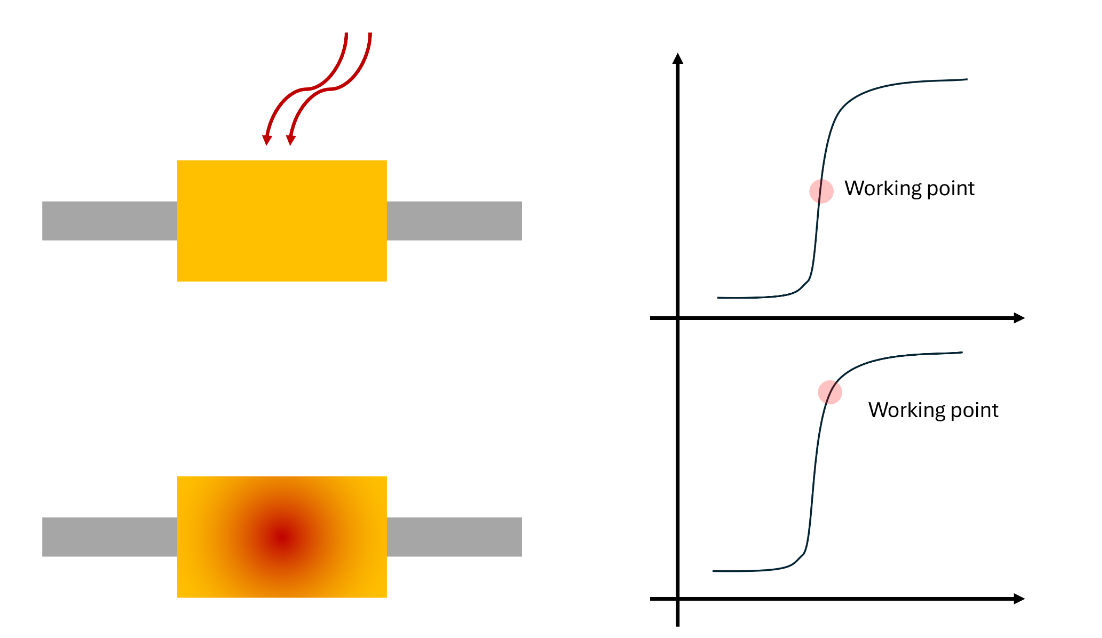
\includegraphics[scale=0.5]{images/TES.png}
	\caption{Simplified diagram of TES operation. When a particle collides with the material and emits a
	phonon, it is absorbed by the TES, which converts all the energy into heat. This raises the temperature
	of the TES, causing its resistance to increase sharply, which produces a detectable signal. }
	\label{tes-diagram}
\end{figure}

Now that we understand how TESs work on a basic level, it is important to discuss how they are realized in a
detector. Specifically, how do we \textit{select} the detection of a particular particle? That is, if we are
interested in detecting WIMPs of a particular energy scale, how do we generate TESs that scan that specific range of
energies? To answer this question, we turn to the \textit{proximity effect}. 


\subsection{The Proximity Effect}
The proximity effect refers to the technique through which experimentalists create superconducting TESs with
a selected \( T_c \). As mentioned, the reason this is desirable is because each particle deposits a
different amount of energy into the TES, so if we are to design a detector to search a particular range of
energies, then we need to engineer our TES so that its thermal response is maximized (or at the very least
detectable) when a particle of that energy collides with the substrate the material. The way this is achieved
is through the \textit{proximity effect}. 

Without going too deep, the idea behind this mechanism is to combine two superconducting metals together
by layering one on top of the other. If the layers are made thin enough, then
the wavefunction that governs the electrons in the superconducting material will be able to "penetrate" the
normal conductor. The overall effect is that we create a superconductor with a \( T_c \) that is between the
\( T_c \) of the initial metals themselves, with its precise value controlled by the ratio of the two metasl
used. 

The exact equations for how this is done is not very important to the central focus of this
thesis. For more information about TESs in general, see \cite{luciaTransitionEdgeSensors2024} for more
information. For now, what matters here is understanding how TESs work, and that it is possible to engineer
these TESs to work under a wide range of conditions by engineering \( T_c \) to the exact temperature we
desire to most easily detect particles of a particular energy. 

\subsection{Readout}

So far, TESs seem to be the perfect kind of detector -- its theoretical principles and the necessary 
engineering techniques are already well developed, and they work for detectors spanning a very wide range of
energies. So why is there even a need for other detection devices? Here, we turn to on
one of the primary "issues" with a TES detector: the way we read out a signal from it. 

As mentioned before, a "signal" from the TES is generated via a change in the resistance of the
superconducting element due to heat, which reads out as a change in current. In the case where we use the TES
as a particle detector, the power \( P_\text{ext} \) delivered to the TES can usually be modeled as a delta 
function \( P_\text{ext} = E_0 \delta(t - t_0) \), and in this regime the current through the TES can be
approximately given by:
\[
	I(t) = -\frac{1}{V} \frac{E_0}{\tau_\text{eff}}e^{-\frac{t}{\tau_\text{eff}}}
	% do you want this here or not?
\]
Again, the specifics of this equation don't really matter too much -- what matters in this equation is
noticing that the amplitude is proportional to \( E_0 \), and since the energy deposited by any particle
colliding with the detector is extremely small the change in \( I(t) \) needs to be amplified in order for it
to be detectable by our experimental instruments. The most popular way this is done is through the use of
Superconducting QUantum Interference Devices (SQUIDs). SQUIDs are electrical circuits that help amplify the
signal of a TES, and in general an array of SQUIDs are generally required to amplify the signal produced by
the TESs in order to get a measurable readout. According to \cite{luciaTransitionEdgeSensors2024}, arrays of
100 SQUIDs are commonplace, which give an output signal of several millivolts. 

The main problem with TESs as they stand is the fact that SQUIDs, which are more or less required, are
relatively complex circuit elements, especially when they are connected together in an array.   
Furthermore, there tends to be many
different sources of noise one needs to consider when designing a SQUID array, which makes them a rather
complex circuit element that requires very special attention. Furthermore, there is the added complication
that due to the complexity of SQUID arrays, it makes them much harder devices to diagnose and fix when a
malfunction occurs. It is these reasons precisely that motivates a new kind of detector that doesn't require
such complex circuitry -- the Kinetic Inductance Detector (KID). 
 

\section{A "New" Device: KID Detectors}
\label{KID}

A Kinetic Inductance Detector (KID) is another kind of detector proposed as an alternative to TESs for dark
matter detection. Unlike TESs, the circuitry involved for a KID-based detector is far simpler than that of a
TES-based one (see \cref{kid-block}), making KIDs a competitive choice as its simplicity makes fixing 
problems with the detector much easier compared to a TES-based detector. 
 
\begin{figure}
	\centering
	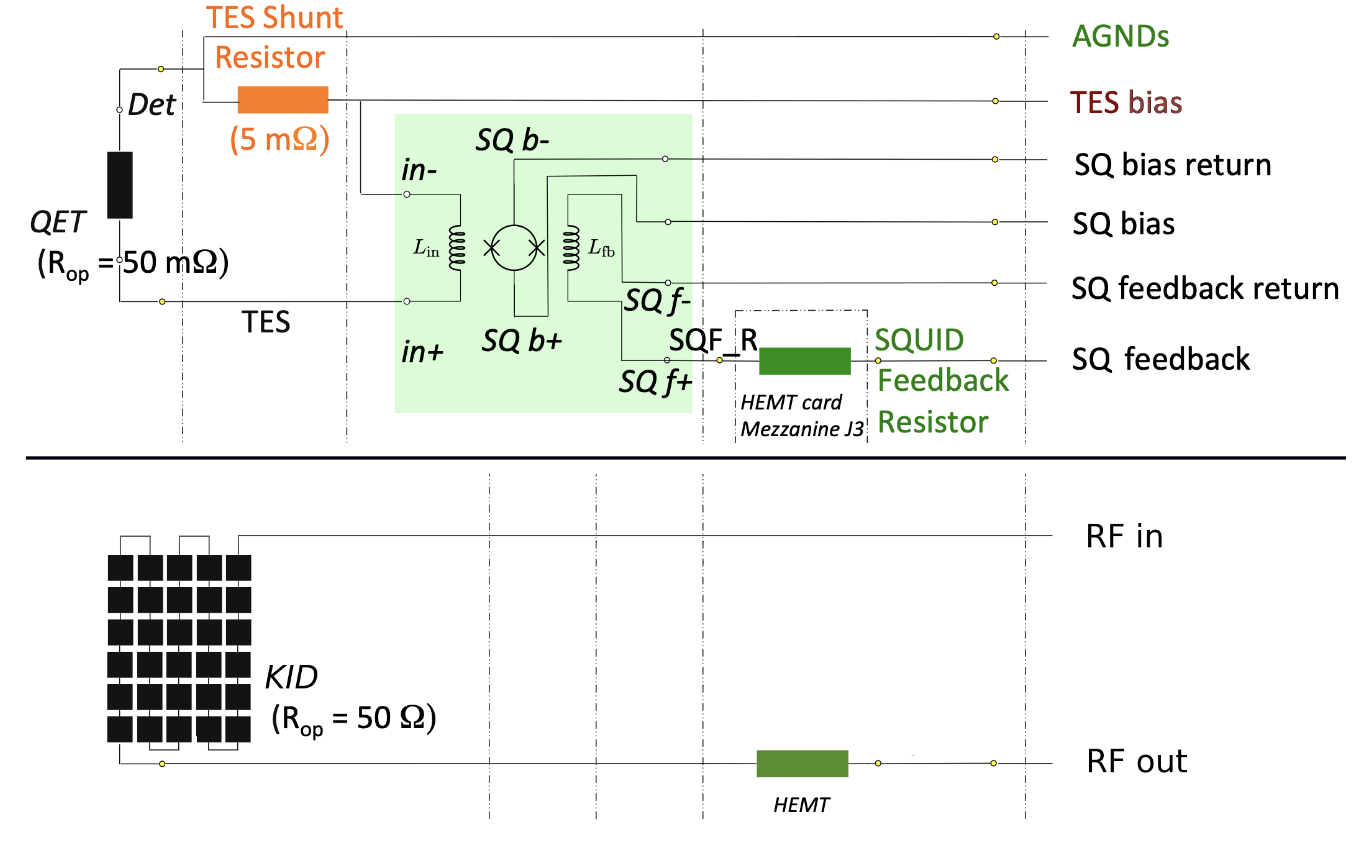
\includegraphics[scale=0.5]{images/kid-circuit.png}
	\caption{Circuit block diagram comparison of a TES-based detector with SQUID amplification (top) compared to
		that of a TES-based detector (bottom). The SQUID amplification circuitry is boxed in green. 
		Of note is the complex circuitry required to calibrate TES readout, whereas no such amplification is needed 
		in principle for a KID-based detector. This diagram is taken from \cite{changSuperCDMSHVeVRun}.}
	\label{kid-block}
\end{figure}

\cref{kid-block} shows a diagrammatic comparison between the circuitry involved in a TES-based detector
with SQUID amplification to that of a KID-based one. As shown in the figure, the SQUID amplification step,
boxed in green in the top diagram, contributes to most of the complexity involved in a TES-based detector. By
comparison, a KID-based detector in principle only requires an RF feedline and an HEMT amplifier to read out
a signal. While both devices require amplification, the HEMT used has been widely commercialized in in the
radio industry, and also requires far less circuitry than SQUIDs. These two factors combine to make a
detector that is much simpler circuitry wise, which makes fixing malfunctions easier while also being
cost-effective.


\subsection{Mechanism}

\begin{figure}
	\centering
	\begin{subfigure}{0.4\textwidth}
		\resizebox{\textwidth}{!}{
		\begin{circuitikz}[scale=2]
			\draw node[left] {\( V \)} (0, 0) to (3, 0);
			\draw (1.5, 0) to[capacitor = \( C_1 \)] (1.5, -0.5);
			\draw (1.5, -0.5) to (1, -0.5) to [vL, a = \( L + L_k \)] (1, -2); 
			\draw (1.5, -0.5) to (2, -0.5) to [capacitor = \( C_2 \)] (2, -2);
			\draw (1, -2) to (2, -2);
			\draw (1.5, -2) to (1.5, -2.5);
			\draw (0, -2.5) node[left] {\( 0 \)} to (3, -2.5);
		\end{circuitikz}
		}
		\caption{}
		\label{kid-circuit}
	\end{subfigure}
	\begin{subfigure}{0.4\textwidth}
		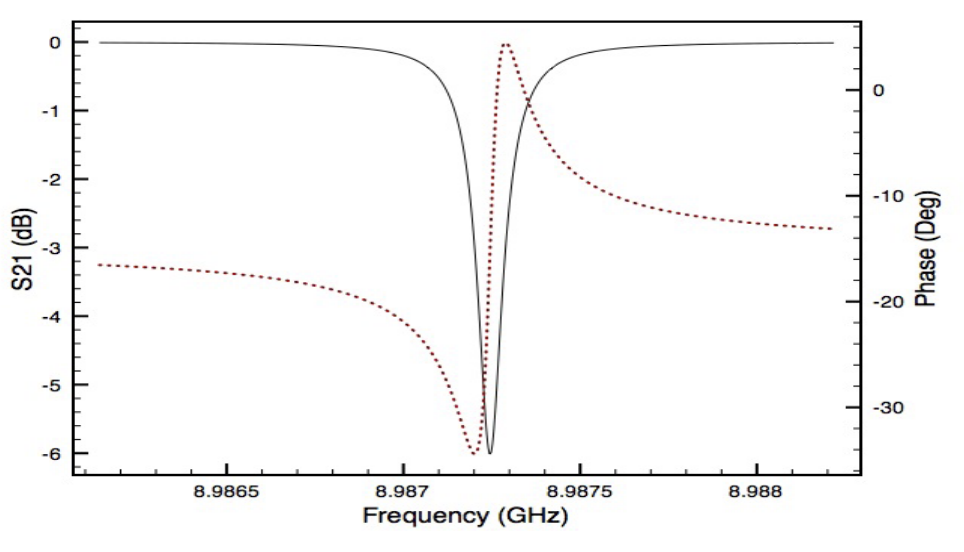
\includegraphics[width = \textwidth, height = 5cm]{images/freq-response.png}
		\caption{}
		\label{freq-response}
	\end{subfigure}
	\caption{(a) circuit schematic of a KID, with the feedline connected at the top and bottom. (b) Example
	frequency response of a KID. Notice the suppression in the signal at all frequencies besides a narrow
band. Figure (b) is taken from \cite{doyleLumpedElementKinetic2008}.} 
\end{figure}

Here, we will go over a high-level overview of how a KID-based particle detector works, much in the same way
we did for TESs earlier. Without going into too much detail, one way to understands KIDs is to model
them as a LC filter as in \cref{kid-circuit}, with the top line set to an AC voltage \( \tilde V \) and the bottom
line acting as a ground. For now, we can imagine the input voltage to be a simple sine wave:
\[
	% do this or do a simple \cos wave
	\tilde V = V_0e^{i (kx - \omega_0 t)}
\]
As a filter, the frequency response of the circuit depends heavily on the frequency \( \omega \), as
shown in \cref{freq-response}. In essence, this means that the amplitude of the output wave depends on that
of the input frequency, in a way where only a narrow band of frequencies are suppressed. In
particular, the resonant frequency of this system is given by:
\[
	\omega = \frac{1}{\sqrt{LC}}
\]
which is the standard formula for the resonant frequency in an LC filter. 
Now, the key to the mechanism is that the inductor in this setup is variable with an
inductance of \( L + L_k \). The value of \( L \) remains fixed, while \( L_k \) is a quantity
that depends on the superconducting characteristics of the KID. 
In particular, when a phonon interacts with a KID, it alters the number of cooper pairs
present, changing the value of \( L_k \), changing its resonant frequency.     
So, the mechanism of operation can be summarized as follows: when a particle interacts with the detector, 
it releases phonons that travel through the substrate. Then, as the phonon interacts with the KID, it
alters the value of \( L_k \), which changes its resonant frequency \( \omega + \delta \omega \) 
by a small amount. Then,
because we never change the input frequency set at \( \omega_0 \), the shift in resonant frequency results in
a change in the output signal which manifests as a pulse, which we record as a detection.  

In a typical detector, we place many such KIDs in series with each other, all connected to the central
transmission line, typically called the "feedline". Because we have intimate control over the inductance 
\( L + L_k \) of each KID, this means we can set each KID to have a slightly different resonant frequency,
allowing us to scan over a wide range of frequencies. We then send in a mixed signal:
\[
	\tilde V = V_0 \sum_i e^{i(kx - \omega_i t)}
\]
where each \( \omega_i \) corresponds to the resonant frequency of each KID in the circuit. If \( \omega_i \)
is chosen correctly, then a phonon detection would only activate one of the KIDs in our array, giving us
information about the energy of the phonon. This can then be extrapolated back to the energy of the particle
fairly easily. 

\section{Focus of Study}
\label{study-focus}
%here talk about waveguides

\begin{figure}
	\centering
	\begin{subfigure}{0.3\textwidth}
		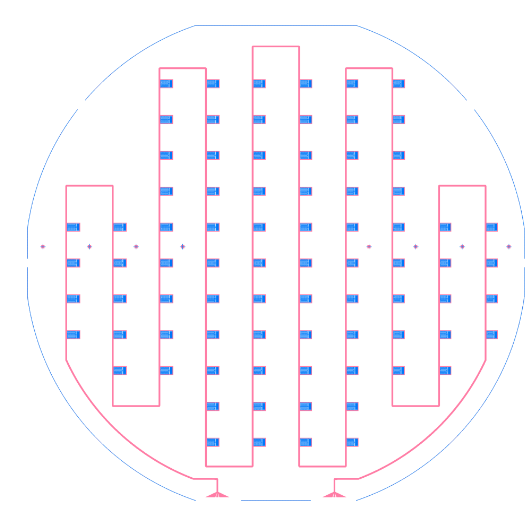
\includegraphics[width=\textwidth]{images/feedline.png}
		\caption{}
		\label{feedline}
	\end{subfigure}
	\hspace{1cm}
	\begin{subfigure}{0.6\textwidth}
		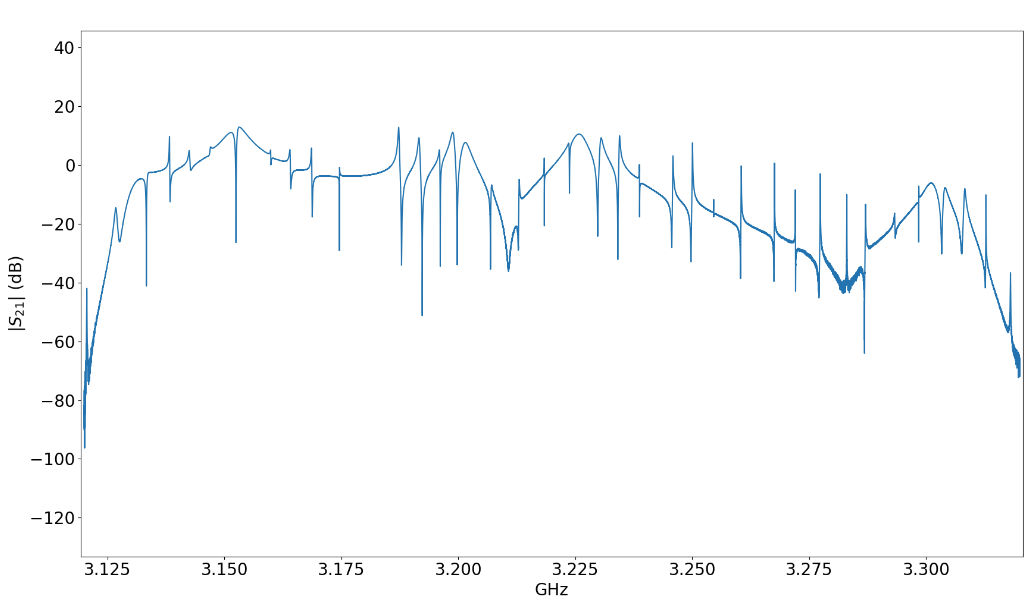
\includegraphics[width=\textwidth]{images/feedline-frequency.png}
		\caption{}
		\label{feedline-freq}
	\end{subfigure}
	\caption{(a) Physical layout of a KID-based detector. Each blue rectangle in the diagram is an individual
	KID, each with a different resonant frequency \( \omega_0 \). (b) Experimental frequency response for
	this KID device. Notice the distortions present in the frequency response as the overall shape is not
	flat, and the attenuation of each KID is nonuniform. Both of these diagrams were sourced from
	\cite{changSuperCDMSHVeVRun}.}
\end{figure}

One aspect of making a successful KID-based detector is the ability to engineer a proper feedline that
minimizes the interference introduced to the KIDs by its presence. To illustrate this point, \cref{feedline}
shows a physical realization of what the KIDs look like on a silicon wafer, and \cref{feedline-freq} shows
its frequency response. The red line in \cref{feedline} is the feedline through which we send in our signal
of mixed sine waves, and each blue rectangle represents an individual KID. The resonant frequency of each KID
is apparent in \cref{feedline-freq}, marked by the numerous sharp spikes present in the frequency response.

In an ideal world, the frequency response should resemble a flat horizontal line, with spikes at even
intervals from the KIDs. However, this is clearly not the case in \cref{feedline-freq} -- not only is the
general shape of the curve not horizontal, but the degree to which each KID attenuates the signal is
nonuniform, which makes pinpointing detections much more difficult. All in all, these effects contribute to
making KIDs an overall weaker detector. It is believed that one of the primary reasons that gives rise to
this effect is the interference caused by introducing a bend in the feedline, which radiates the supposiedly
KID-reading signal to excite the box's resonant cavity modes, which in turn couple to the KID resonances and
heavily affect the detector's designed performance. 

The focus of my thesis is to verify, through simulation, the validity of this claim. Originally, the focus of
this thesis was to investigate the use of a slow-wave structure proposed in
\cite{hosaengkimWireBondFreeTechnique2009}, but I was not able to fully investigate that effect in time for
this thesis. Instead, we focus on the feedline itself, seeking to investigate which particular factors in the
feedline's design affect its transmission the most.    


 


% articulate the problem here.
 
  
     


